%----------------------------------------------------------------------------------------
%	PACKAGES AND OTHER DOCUMENT CONFIGURATIONS
%----------------------------------------------------------------------------------------

\documentclass[
11pt, % Main document font size
a4paper, % Paper type, use 'letterpaper' for US Letter paper
oneside, % One page layout (no page indentation)
%twoside, % Two page layout (page indentation for binding and different headers)
pdfspacing, % Makes use of pdftex’ letter spacing capabilities via the microtype package
headinclude,
%footinclude, % Extra spacing for the header and footer
BCOR5mm, % Binding correction
ngerman, %set document to German
bibtotocnumbered,
]{scrartcl}
%{scrartcl}

%%%%%%%%%%%%%%%%%%%%%%%%%%%%%%%%%%%%%%%%%
% Arsclassica Article
% Structure Specification File
%
% This file has been downloaded from:
% http://www.LaTeXTemplates.com
%
% Original author:
% Lorenzo Pantieri (http://www.lorenzopantieri.net) with extensive modifications by:
% Vel (vel@latextemplates.com)
%
% License:
% CC BY-NC-SA 3.0 (http://creativecommons.org/licenses/by-nc-sa/3.0/)
%
%%%%%%%%%%%%%%%%%%%%%%%%%%%%%%%%%%%%%%%%%

%----------------------------------------------------------------------------------------
%	REQUIRED PACKAGES
%----------------------------------------------------------------------------------------

\usepackage[usenames,dvipsnames]{color} % Required for specifying custom colors and referring to colors by name

\usepackage[
nochapters, % Turn off chapters since this is an article        
beramono, % Use the Bera Mono font for monospaced text (\texttt)
%eulermath,% Use the Euler font for mathematics
eulerchapternumbers,
pdfspacing, % Makes use of pdftex’ letter spacing capabilities via the microtype package
dottedtoc % Dotted lines leading to the page numbers in the table of contents
]{classicthesis} % The layout is based on the Classic Thesis style

%\usepackage{arsclassica} % Modifies the Classic Thesis package

\usepackage[T1]{fontenc} % Use 8-bit encoding that has 256 glyphs

\usepackage[utf8]{inputenc} % Required for including letters with accents

\usepackage{graphicx} % Required for including images
\graphicspath{{Figures/}} % Set the default folder for images

\usepackage{enumitem} % Required for manipulating the whitespace between and within lists

\usepackage{lipsum} % Used for inserting dummy 'Lorem ipsum' text into the template

\usepackage{amsmath,amssymb,amsthm} % For including math equations, theorems, symbols, etc

\usepackage{varioref} % More descriptive referencing

\usepackage{url}

\usepackage{hyperref}

\usepackage{gensymb}	%for the \degree command

\usepackage[ngerman, english]{babel}

\usepackage[square,
authoryear,
%numbers,
longnamesfirst
]{natbib}

\usepackage{enumitem}

\usepackage{authblk}

\usepackage{relsize, etoolbox, lmodern}% http://ctan.org/pkg/{relsize,etoolbox}

\AtBeginEnvironment{quote}{\smaller\fontfamily{lmss}\selectfont}% Step font down one size relative to current font.
% see http://tex.stackexchange.com/questions/25249/how-do-i-use-a-particular-font-for-a-small-section-of-text-in-my-document for fontfamilies

\usepackage{chngcntr}

% to have a separation in the text with extra space between paragraphs and no indendation following
\newcommand*{\skippingparagraph}{\par\vspace{1.0\baselineskip}\noindent}

%----------------------------------------------------------------------------------------
%	HYPERLINKS
%---------------------------------------------------------------------------------------
\definecolor{mediumviolet-red}{rgb}{0.78, 0.08, 0.52}
\hypersetup{
%	draft, % Uncomment to remove all links (useful for printing in black and white)
	colorlinks=true, breaklinks=true, bookmarks=true,bookmarksnumbered,
	urlcolor=webbrown, linkcolor=mediumviolet-red, citecolor=webgreen, % Link colors
	pdftitle={}, % PDF title
	pdfauthor={\textcopyright}, % PDF Author
	pdfsubject={}, % PDF Subject
	pdfkeywords={}, % PDF Keywords
	pdfcreator={pdfLaTeX}, % PDF Creator
	pdfproducer={LaTeX with hyperref and ClassicThesis} % PDF producer
}

%----------------------------------------------------------------------------------------
%	TODONOTES
%---------------------------------------------------------------------------------------

\usepackage[colorinlistoftodos]{todonotes}

\newcommand{\todoInfo}[1]{\todo[color=blue!25]{INFO: #1}}
\newcommand{\todoCite}[1]{\todo[color=green!40]{INFO: #1}}


%----------------------------------------------------------------------------------------
%	CODESNIPPETS
%---------------------------------------------------------------------------------------

%%%%%%%%%%%%%%%%%%%%%%%%%%%%%%%%%%%%%%%%%
% Code Snippet
% LaTeX Template
% Version 1.0 (14/2/13)
%
% This template has been downloaded from:
% http://www.LaTeXTemplates.com
%
% Original author:
% Velimir Gayevskiy (vel@latextemplates.com)
%
% License:
% CC BY-NC-SA 3.0 (http://creativecommons.org/licenses/by-nc-sa/3.0/)
%
%%%%%%%%%%%%%%%%%%%%%%%%%%%%%%%%%%%%%%%%%
\usepackage{listings} % Required for inserting code snippets

\definecolor{DarkGreen}{rgb}{0.0,0.4,0.0} % Comment color
\definecolor{highlight}{RGB}{255,251,204} % Code highlight color
\definecolor{DogwoodRose}{rgb}{0.84, 0.09, 0.41}
\definecolor{lemonchiffon}{rgb}{1.0, 0.98, 0.8}
\definecolor{lightgoldenrodyellow}{rgb}{0.98, 0.98, 0.82}
\definecolor{oldlace}{rgb}{0.99, 0.96, 0.9}
\definecolor{oldlavender}{rgb}{0.47, 0.41, 0.47}
\definecolor{pakistangreen}{rgb}{0.0, 0.4, 0.0}
\definecolor{ao}{rgb}{0.0, 0.0, 1.0}
\definecolor{britishracinggreen}{rgb}{0.0, 0.26, 0.15}
\definecolor{coquelicot}{rgb}{1.0, 0.22, 0.0}
\definecolor{cordovan}{rgb}{0.54, 0.25, 0.27}
\definecolor{darkcandyapplered}{rgb}{0.64, 0.0, 0.0}
\definecolor{mediumchampagne}{rgb}{0.95, 0.9, 0.67}

\lstdefinestyle{Style1}{ % Define a style for your code snippet, multiple definitions can be made if, for example, you wish to insert multiple code snippets using different programming languages into one document
	language=JavaScript, % Detects keywords, comments, strings, functions, etc for the language specified
	backgroundcolor=\color{oldlace}, % Set the background color for the snippet - useful for highlighting
	basicstyle=\smaller\smaller\ttfamily, % The default font size and style of the code
	breakatwhitespace=true, % If true, only allows line breaks at white space
	breaklines=true, % Automatic line breaking (prevents code from protruding outside the box)
	captionpos=b, % Sets the caption position: b for bottom; t for top
	commentstyle=\usefont{T1}{pcr}{m}{sl}\color{ao}, % {m}DarkGreen Style of comments within the code - dark green courier font
	deletekeywords={}, % If you want to delete any keywords from the current language separate them by commas
	%escapeinside={\%}, % This allows you to escape to LaTeX using the character in the bracket
	firstnumber=1, % Line numbers begin at line 1
	frame=single, % Frame around the code box, value can be: none, leftline, topline, bottomline, lines, single, shadowbox
	frameround=tttt, % Rounds the corners of the frame for the top left, top right, bottom left and bottom right positions
	keywordstyle=\color{darkcandyapplered}\textbf, % Functions are bold and blue
	morekeywords={}, % Add any functions no included by default here separated by commas
	numbers=left, % Location of line numbers, can take the values of: none, left, right
	numbersep=10pt, % Distance of line numbers from the code box
	numberstyle=\tiny\color{Gray}, % Style used for line numbers
	rulecolor=\color{black}, % Frame border color
	showstringspaces=false, % Don't put marks in string spaces
	showtabs=false, % Display tabs in the code as lines
	stepnumber=5, % The step distance between line numbers, i.e. how often will lines be numbered
	stringstyle=\color{Purple}, % Strings are purple
	tabsize=2, % Number of spaces per tab in the code
}

\definecolor{darkgray}{rgb}{.4,.4,.4}
\definecolor{purple}{rgb}{0.65, 0.12, 0.82}


%define Javascript language
\lstdefinelanguage{JavaScript}{
	keywords={typeof, new, true, false, catch, try, finally, function, return, null, then, catch, switch, var, if, in, while, do, else, case, break, yield, async, await},
	keywordstyle=\color{blue}\bfseries,
	ndkeywords={class, export, boolean, throw, implements, import, this},
	ndkeywordstyle=\color{darkgray}\bfseries,
	identifierstyle=\color{black},
	sensitive=false,
	comment=[l]{//},
	morecomment=[s]{/*}{*/},
	commentstyle=\color{purple}\ttfamily,
	stringstyle=\color{red}\ttfamily,
	morestring=[b]',
	morestring=[b]"
}

\lstset{
	language=JavaScript,
	extendedchars=true,
	basicstyle=\footnotesize\ttfamily,
	showstringspaces=false,
	showspaces=false,
	numbers=left,
	numberstyle=\footnotesize,
	numbersep=9pt,
	tabsize=2,
	breaklines=true,
	showtabs=false,
	captionpos=b
}

% Create a command to cleanly insert a snippet with the style above anywhere in the document
\newcommand{\insertcode}[2]{\begin{itemize}\item[]\lstinputlisting[{caption={#2}},label=#1,style=Style1]{#1}\end{itemize}} % The first argument is the script location/filename and the second is a caption for the listing
 % Include the structure.tex file which specified the document structure and layout
%----------------------------------------------------------------------------------------
%	TITLE AND AUTHOR(S)
%----------------------------------------------------------------------------------------
\selectlanguage{ngerman}

\subtitle{\normalfont{Fachpraktikum 1597 an der FernUni Hagen im SS 2017:\protect\\Parallele Programmierung }}

\title{\normalfont{Vorgehensweise zur Erkennung von möglichen Notlandefeldern aus Höhendaten mittels POSIX Thread Implementation}} % The article title
%\title{\normalfont\spacedallcaps{Asnychrone Programmierung: \protect\\ Moderne Methoden in ECMAScript~6}} % The article title



\author{Felix Eckstein*, Dr. Björn Wittich**} % The article author(s) 

\date{Juni 2017} % An optional date to appear under the author(s)

%----------------------------------------------------------------------------------------

\begin{document}
	
	\maketitle % Print the title/author/date block

	\tableofcontents % Print the table of contents

	
	{\let\thefootnote\relax\footnotetext{* \textit{Student im Bachelor of Science Informatik an der FernUniversität Hagen,\protect\\Matr.-\#: 8161569, \href{mailto:felix.eckstein@gmx.de}{felix.eckstein@gmx.de}}}}
	{\let\thefootnote\relax\footnotetext{** \textit{Student im Bachelor of Science Informatik an der FernUniversität Hagen,\protect\\Matr.-\#: 9265953, \href{mailto:BjoernWittich@gmx.de}{BjoernWittich@gmx.de}}}}
	
	\selectlanguage{ngerman}

\section{Vorgehensweise zur Erkennung von möglichen Notlandefeldern aus Höhendaten}

	\subsection{Grundsätzliche Überlegungen}
	
	
	\subsection{Kriterien für geeignete Notlandeflächen}
	
	Zunächst muss definiert werden, was eine geeignete Landefläche ausmacht und wie sie charakterisiert werden kann. Es ist sofort einsichtig, dass eine Landebahn auf einer ausreichend großen Fläche glatt und eben sein muss. Die Fläche wird durch eine Mindestlänge und eine Mindestbreite charakterisiert. Daraus ergibt sich auch direkt eine Richtung. Als globale Parameter einer Landebahn sind also folgende Daten festzuhalten:
	\begin{itemize}
		\item Richtung der Bahn
		\item Breite
		\item Länge
	\end{itemize}

	Das Kriterium "`glatt und eben"' muss weiter spezifiziert werden. Dazu bieten sich Steigungskriterien an:
	
	\paragraph{Charakterisierung durch Steigungsdaten}
	Eine Landebahn kann durch einen Satz von Steigungsdaten charakterisiert werden:
	\begin{itemize}
		\item "`global"': Eine Landebahn darf auf Ihrer gesamten Länge nicht über ein gewisses Maß hinaus ansteigen. Ein Flugzeug kann nicht zu stark bergauf und auch nicht bergab landen. Es muss also für die gesamte minimale Bahnlänge ein maximaler Anstieg und ein maximaler Abfall vorgegeben werden.
		\item "`lokal"': Für (deutlich) kürzere Strecken als die Gesamtbahnlänge ist ein anderer Satz von maximalen/minimalen Steigungslimits notwendig, welche die maximale "`Holprigkeit"' der potentiellen Bahn beschreiben.
		\item "`Querneigung"': Eine optimale Landebahn ist senkrecht zur langen Achse perfekt eben. Eine reale Bahn darf geneigt bzw. in sich "`verwunden"' sein, solange kein kritischer Grenzwert für diese Querneigung überschritten wird. Diese maximale Querneigung wird über die Mindestbreite der Bahn angegeben.
		\item "`Verwindung"': Die Änderung der Querneigung darf sicherlich ein bestimmtes Limit nicht überschreiten. Es sollte also nicht die maximale "`Linksneigung"' direkt auf die maximale "`Rechtsneigung"' folgen.
%		TODO: Bei diesem Kriterium müssen wir uns nochmal überlegen, ob wir das tatsächlich mit aufnehmen wollen. Ist aber auch nicht schwierig zu implementieren. 
	\end{itemize}

	Das globale Limit der Steigung ist sicherlich geringer als das lokale Limit für die Holprigkeit. (Extremfall: Landen auf Kopfsteinpflaster kann lokal ziemlich große Steigungen verursachen, wenn das Raster klein genug ist, stellt aber eigentlich kein Problem dar, da die Strecken zwischen den Rasterpunkten kurz genug sind.)
	
	\skippingparagraph
	\fbox{\begin{minipage}{\textwidth}
			{\bfseries\textsf{notwendige Eingabedaten:}}
			
			Um aus den Höhendaten geeignete Landebahnen zu ermitteln, bekommt der zu beschreibende Algorithmus folgende Eingabedaten:
			\begin{itemize}
				\item minimale Bahnlänge in Metern
				\item Breite der Bahn in Metern
				\item Richtung der Bahn in Grad
				\item "`Holprigkeitslimit"': maximale Steigung im kurzen Bereich. Angegeben durch Höhendifferenz und Länge jeweils in Metern.
				\item "`Gesamtsteigung"': maximaler Anstieg und maximaler Abfall über die angegebene minimale Bahnlänge in Metern
				\item "`Querneigung"': maximale Querneigung der Bahn. Angegeben durch Höhendifferenz in Metern über der gewünschten Bahnbreite.
				\item "`Verwindung"': Die maximale Änderungsrate der Querneigung angegeben in Prozent pro Meter in Hauptrichtung.
			\end{itemize}
	\end{minipage}}


	\paragraph{Offene Punkte:} 
	\begin{itemize}
		\item Muss die Holprigkeit in Querrichtung vollständig geprüft werden, oder reicht es aus die maximale Querneigung über die (relativ kurze) Bahnbreite zu betrachten?
		\item Sind verschiedene Holprigkeitslimits in Längs- und in Querrichtung notwendig?
		\item Ist es notwendig "`Zwischenlängen"' passend zu ergänzen? Z. B. indem eine kürzere Länge so lange verdoppelt wird, bis sich die nächst längere Länge ergibt. Dann müsste ein "`gewichteter"' Mittelwert der erlaubten maximalen Steigungen angegeben werden, damit eine Gesamtsteigung mit einem überlagerten "`Holpern"' noch OK ist. 
	\end{itemize}
	Diese offenen Punkte werden in der Erprobung sicherlich klar werden.


\section{Datenbasis}

Die Höhedaten liegen in Form eines GeoTIFF Formats vor. Dabei handelt es sich um ein Rasterformat, bei dem jedem Rasterpunkt bestimmte Geodaten zugeordnet werden. Diese Daten werden in dem Grafikformat anstelle der normalerweise enthaltenen Farbwerte gespeichert und müssen entsprechend ihrer Bedeutung interpretiert werden. Prinzipiell ist es möglich mehrere Werte pro Rasterpunkt zu speichern. In unserem Fall ist für jeden Rasterpunkt die Höhe über normal Null in Metern angegeben. Dieser Wert liegt als einfach genaue 32bit Gleitkommazahl vor.

Für die Kodierung und Komprimierung der Werte wird das bekannte TIFF Format eingesetzt, das insbesondere auch die verlustlose Speicherung unterstützt.

Zusätzlich zu dem in einer TIFF-Datei eingebetteten Nutzdatensatz gehören zu einem GeoTIFF noch Angaben über Auflösung und Projektion des Datensatzes. Damit wird es möglich, jedes Pixel des GeoTIFF eindeutig einem Punkt auf der Erdoberfläche in den üblichen Koordinaten aus geographischer Länge und Breite zuzuordnen.

Für die ersten Experimente und die Validierung des Verfahrens wird ein Höhendatensatz von Nordrhein-Westfalen verwendet. Dieser ist verfügbar unter \href{http://data.opendataportal.at/dataset/dtm-germany/resource/08d8c183-a4cc-4a7b-84a0-d03f92076ed3}{DTM Germany\textunderscore Nordrhein-Westfalen, 20m}


	\subsection{Auflösung}
	Ob der zu entwickelnde Algorithmus zum Auffinden von möglichen Notlandefeldern in der Praxis tauglich ist, hängt wesentlich von der Qualität und Auflösung der Eingabedaten ab. Der vorliegende Datensatz hat eine horizontale Auflösung von 20m und eine vertikale Auflösung von 0.1m. 
	
	Intuitiv wird eine 20m Auflösung für die Bestimmung der Holprigkeit einer Bahn zu grob sein. 
	
	Es ist angekündigt, dass im weiteren Verlauf dieses Praktikums ein deutlich höher aufgelöster Datensatz zur Verfügung gestellt werden kann. Dies ist bei der Auslegung der Algorithmen und Berechnungsmethoden von Anfang an einzuplanen. Dabei ist zu beachten, dass die Datenmenge quadratisch mit der Auflösung wächst. Ein mit 1m horizontal aufgelöster Datensatz ist also schon 400 Mal so groß wie der vorliegende Testdatensatz.
	
	\subsection{Dateneinlesung}
	Für das Einlesen der Daten kann auf bewährte OpenSource Tools zurückgegriffen werden. Diese müssen für den speziellen Einsatzzweck angepasst, aber nicht von Grund auf neu entwickelt werden.
	
	Die Einlesung der Rasterdaten kann mit einer angepassten Version von \href{https://www.imnc.in2p3.fr/pagesperso/deroulers/software/largetifftools/tifffastcrop.html}{tifffastcrop} erfolgen\footnote{
	Details dazu siehe: Deroulers et al., \href{https://www.imnc.in2p3.fr/pagesperso/deroulers/software/ndpitools/article_diagnostic_pathology.pdf}{Analyzing huge pathology images with open source software}, \href{http://www.diagnosticpathology.org/content/8/1/92}{Diagnostic Pathology 8:92 (2013)}}. 
	Dies hat im Prototypen problemlos funktioniert.
	
	Beim Einlesen ist darauf zu achten, dass ein effizientes Verfahren zum Einlesen von Kacheln notwendig ist, da bei höher aufgelösten Daten nicht mehr davon ausgegangen werden kann, dass alle Daten auf einmal im RAM gehalten werden können.
	
	Zur Umrechnung der Pixelkoordinaten in geographische Koordinaten und zur Ermittlung der Metadaten des GeoTIFF Datensatzes kann auf \href{https://trac.osgeo.org/geotiff/}{libgeotiff} zurückgegriffen werden.
	
	\skippingparagraph
	\fbox{\begin{minipage}{\textwidth}
			{\bfseries\textsf{Einlesen der Eingabedaten:}}
			
			Als Anforderung an die Einlesung der Eingabedaten ergibt sich:
			\begin{itemize}
				\item Es müssen nacheinander Kacheln mit Rücksicht auf vorhandene Speicherbelegung eingelesen werden können
				\item Die Metadaten (Auflösung des Datensatzes, Ausdehung der Daten) müssen bereit gestellt werden
				\item Routinen zur Umrechnung von/in Pixelkoordinaten von/in geographische Koordinaten müssen bereit gestellt werden.
			\end{itemize}
	\end{minipage}}
	\skippingparagraph	%Offensichtlich muss nach der Minipage noch etwas kommen, sonst kommt TeXStudio mit der Struktur durcheinander.
	
	

\section{Durchmusterung}

Die zentrale Funktion zum Auffinden von Notlandebahnen ist eine systematische Durchmusterung der eingelesenen Daten. Obwohl diese Funktion im Grundsatz sehr trivial scheint, so ergeben sich doch einige beachtenswerte Details, die nachfolgend angegeben werden sollen.

\subsection{Einfache Durchmusterung}\label{Einfache_Durchmusterung}
Eine Landebahn kann auf jedem beliebigen Rasterpunkt der Höhendaten beginnen. Von einem Startpunkt ausgehend muss in einer geraden Richtung ein Bereich existieren, in dem keines der angegebenen Kriterien verletzt wird. 

Eine geeignete Landebahn ist gefunden, wenn ein rechteckiger Bereich gefunden ist, bei dem für jeden Rasterpunkt innerhalb der minimalen geforderten Länge und Breite die gegebenen Steigungslimits nicht überschritten werden.
Auch wenn die kürzeste Vorausschaulänge länger ist als der Abstand der Rasterpunkte, so muss die Überprüfung der Steigungslimits doch für jeden Rasterpunkt innerhalb der Bahn erfolgen und entsprechend positiv ausfallen.

Der Algorithmus zur Durchmusterung eines Datensatzes muss also von jedem vorhandenen Rasterpunkt in vorgegebener Richtung die Kriterien abtesten und festhalten, ob ein bestimmter Punkt als Startpunkt einer Landebahn in Frage kommt.

Eine Kachel wird so groß gewählt, dass sie vollständig in den Speicher passt und zusätzlich Platz ist, für die einzelnen Punkte alle notwendigen Verwaltungs- und Ergebnisinformationen zu speichern.

Eine Kachel wird in jedem Durchgang auf Bahnen in einer vorgegebenen Richtung durchmustert. Diese Richtung gibt die Längsachse der potentiellen Bahn an.

Die Steigungsüberprüfung erfolgt immer vorwärts gerichtet und berechnet den Quotienten aus Höhenänderung über Vorausschaulänge. Es wird also überprüft, ob vom aktuellen Punkt aus vorwärts kein Hindernis eine Landung unmöglich macht.

	\skippingparagraph
	\fbox{\begin{minipage}{\textwidth}
		{\bfseries\textsf{Brute Force:}}
		\begin{itemize}
			\item Berechne für jeden Punkt die Steigungsmaße für die vorgegebenen Vorausschaulängen und speichere sie pro Punkt.
			\begin{itemize}
				\item Gesamtsteigung
				\item Holprigkeit
				\item Querneigung
				\item Verwindung
			\end{itemize}
			\item Wenn ein Limit gerissen wurde, dann markiere das entsprechend.
			\item Gehe zum nächsten Punkt.
		\end{itemize}
	
		Alle Punkte, die sämtliche Steigungstests bestehen sind Kandidatenpunkte für den Beginn einer Landebahn.
		\begin{itemize}
			\item Fasse die Kandidatenpunkte von einem potentiellen Startpunkt entlang der Durchmusterungsrichtung in möglichst lange Teilstrecken zusammen.
			\item Streiche alle Teilstrecken kürzer als die Mindestbahnlänge
		\end{itemize}
	
		Beachte: Ein Punkt kann durchaus innerhalb einer Landebahn liegen, auch wenn er nicht Startpunkt einer Bahn sein kann. Jedes Kriterium hat eine eigene Vorausschaulänge. Ein Punkt muss nur dann endgültig ausgeschlossen werden, wenn die Kriterien gerissen wurden, deren Vorausschaulänge vollständig innerhalb der potentiellen Landebahn liegt.\footnote{Beispiel: Ein Punkt muss als Startpunkt ausgeschlossen werden, da von ihm aus betrachtet das Gesamtsteigungskriterium über ein komplette Bahn überschritten wird. Dieser Punkt kann aber trotzdem Bestandteil in der Mitte einer Landebahn sein solange seine Kriterien mit kürzerer Vorausschau (Holprigkeit) und seine lokalen Kriterien (Querneigung, Verwindung) dies nicht unmöglich machen.}
	\end{minipage}
}

	\skippingparagraph	%Offensichtlich muss nach der Minipage noch etwas kommen, sonst kommt TeXStudio mit der Struktur durcheinander.
 

\subsection{Berücksichtigung unterschiedlicher Rasterweiten}

	Die Durchmusterung muss mit allen möglichen Rasterweiten zurechtkommen. Der Durchmusterungsalgorithmus muss also so programmiert werden, dass die Rasterweite keine Rolle spielt. Der Algorithmus soll auch in der Lage sein, in horizontaler und in vertikaler Richtung mit unterschiedlichen Rasterweiten zurechtzukommen. Die Rasterweiten (in Metern) müssen von der Dateneinleseroutine in X- und Y-Richtung bereitgestellt werden.

	Dazu sind folgende Überlegungen anzustellen:
	
 	\begin{minipage}{\textwidth}
 		\skippingparagraph
 		
		\begin{minipage}[t]{\textwidth-4cm}
			\vspace{0pt}
			Bei rechteckigen Rastern stimmt die Rasterrichtung nur in Ausnahmefällen mit der Durchmusterungsrichtung überein. Um sicher zu sein, dass die Landebahn an jeder Stelle die benötigten Kriterien erfüllt muss jedes Rasterpixel untersucht werden, das vom Durchmusterungsstrahl berührt wird. Ausgehend von einem Pixel wird der Strahl in die gewünschte Richtung über das Raster geworfen und jedes Pixel, das berührt wird muss als Prüfpunkt benutzt werden.
			
			Analog müssen die Pixel senkrecht zur gewählten Durchmusterungsrichtung ausgewählt werden um die Querneigung und Verwindung zu prüfen.
			
			In der nebenstehenden Grafik ist dies grafisch verdeutlicht.
		\end{minipage}
		\begin{minipage}[t]{3cm}
			\vspace{0pt}
			\centering
			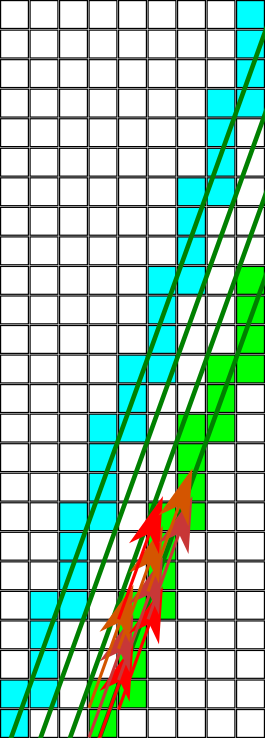
\includegraphics{./drawings/Durchmusterungspfad.png}
		\end{minipage}
	\skippingparagraph
	\end{minipage}
	
	
	
	Das Holprigkeitskriterium hat die kürzeste Vorausschaulänge. Es sind zwei Fälle zu unterscheiden: 
	
	Entweder ist die Vorausschaulänge kürzer als der Abstand zweier Pixel, oder die Vorausschaulänge ist mindestens so lang wie der aktuelle Pixelabstand.
	
	Bei Pixelabständen, die größer sind als die aktuelle Vorausschaulänge muss die Vorausschaulänge künstlich auf den Pixelabstand in Durchmusterungsrichtung erhöht werden. Die zugehörige Höhendifferenz muss entsprechend skaliert werden. 
	
	 	\begin{minipage}{\textwidth}
		\skippingparagraph
		
		\begin{minipage}[t]{3cm}
			\vspace{0pt}
			\centering
			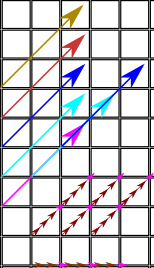
\includegraphics[width=3cm]{./drawings/Vorausschaulaengen.png}
		\end{minipage}
			\begin{minipage}[t]{\textwidth-3cm}
				\vspace{0pt}
				Bei Pixelabständen, die kleiner oder gleich der aktuellen Vorausschaulänge sind, wird die Steigung aus der Höhendifferenz zwischen Start- und der Zielpixel berechnet. Eine Skalierung muss nicht stattfinden. Es ist aber zu beachten, dass entlang des Durchmusterungspfades jedes Pixel als Startpunkt betrachtet werden muss.			
		\end{minipage}\skippingparagraph
	\end{minipage}

	Bei Vorausschaulängen, die kürzer sind als die aktuelle Rasterweite, kann das vorgestellte Verfahren dazu führen, dass Hindernisse übersehen werden die vollständig innerhalb einer Kachel liegen oder die wegen der Skalierung der Steigung als zulässig angesehen werden, obwohl sie in der Realität zu hoch sind. Eine Interpolation innerhalb der Kacheln würde jedoch auch nichts nützen, da die Eingangsdaten einfach "`nicht mehr hergeben"'. Somit scheint das vorgeschlagene Vorgehen der beste Kompromiss zur Vorauswahl geeigneter Landeflächen zu sein. Bei ernsthafter Anwendung werden besser aufgelöste Daten benötigt.
	
	\skippingparagraph
	
	Um die vollständige im Speicher befindliche Kachel zu durchmustern, muss der Durchmusterungsstrahl viele Male über die Kachel geworfen werden. Die Kacheln im Speicher sind immer rechteckig. Die gesamte Fläche soll mit Durchmusterungsstrahlen überdeckt werden. Diese einzelnen Strahlen sollten untereinander einen Abstand von 1 Pixel haben. Bei nicht quadratischen Pixeln ist der Pixelabstand in der Hauptrichtung als relevanter Strahlabstand zu benutzen.
	
	Die Strahlen können dazu immer vom unteren bzw. linken Rand der im Speicher befindlichen Kachel ausgehen. Die tatsächliche Durchmusterung findet natürlich nur in dem Bereich statt, in dem der Strahl über Pixeln der Kachel verläuft.
	
	Im hier gezeigten Beispiel läuft die Durchmusterung in Richtung 19,8\degree nach Nord-Nord-Ost. Die Auflösung des Rasters betrage 2,5m. Dann sollen die parallelen Durchmusterungsstrahlen einen Abstand von 2,5m untereinander haben. Das ergibt einen auf die horizontale Grundlinie projizierten Abstand von $\frac{2.5m}{\cos 19.8\degree} = 2,657m$
	
	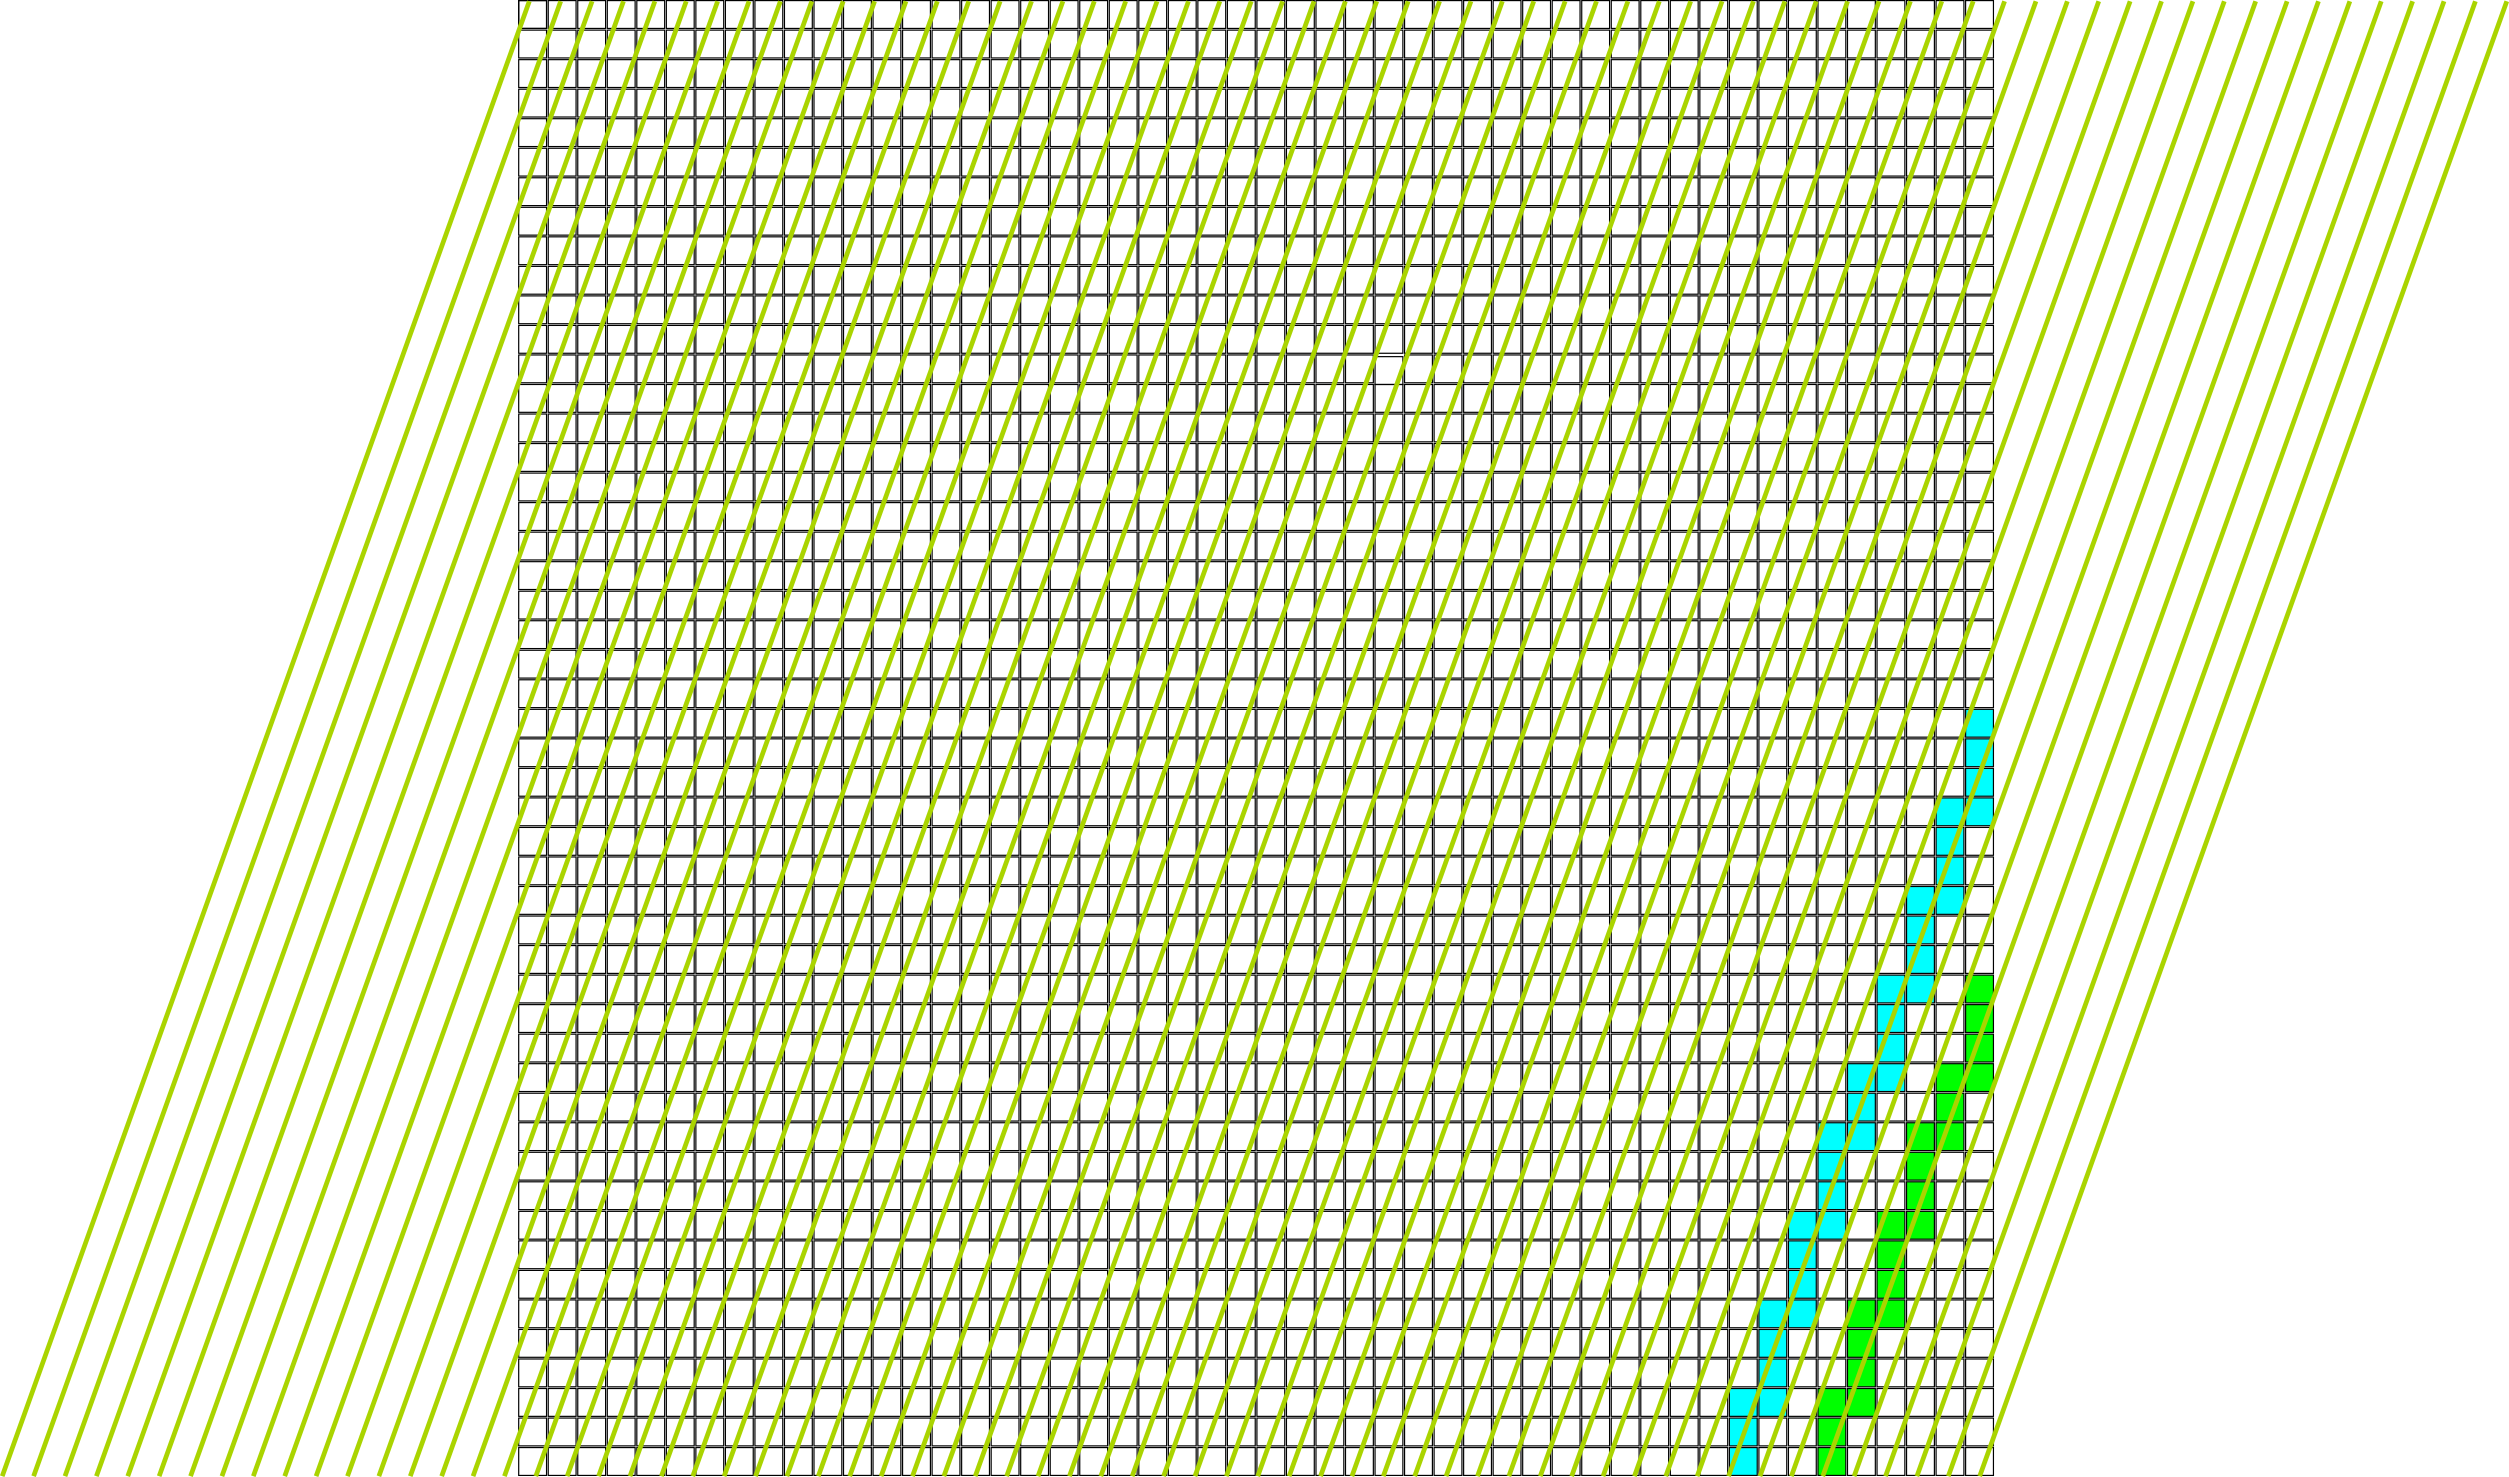
\includegraphics[width=\textwidth]{./drawings/Durchmusterungspfade_schraeg.png}
	
	Bei sehr feinen Rastern ist es sicherlich sinnvoll nach unten einen bestimmten Abstand nicht zu unterschreiten (z. B. 1m) um den Aufwand nicht ausufern zu lassen. Die Gefahr, dass dadurch eine potentielle Landebahn übersehen wird scheint intuitiv eher gering.

	

\subsection{Optimierung}

Das vorgestellte Verfahren geht stumpf über jeden Punkt der Daten und versucht dann zusammenhängende geeignete Punkte zu erkennen. Bei den zu erwartenden großen (weil hochaufgelösten) Datensätzen sollten soviele Punkte wie möglich so früh wie möglich ausgeschlossen werden um den Rechenaufwand so gering wie möglich zu halten.

Idee zur Optimierung:

Um die Menge der (genau) zu überprüfenden Daten möglichst schnell zu minimieren, ist es wichtig, dass bei einem frühen Durchlauf schon möglichst viele Punkte als Kandidaten herausfallen.

Wenn ein Punkt aus der Kandidaten Menge herausfällt, dann wirft er einen „Schatten“ auf das zurückliegende Stück. Eine Bahn kann nicht geeignet sein, wenn sie innerhalb ihrer Mindestlänge diesen ungeeigneten Punkt zwangsläufig enthält.

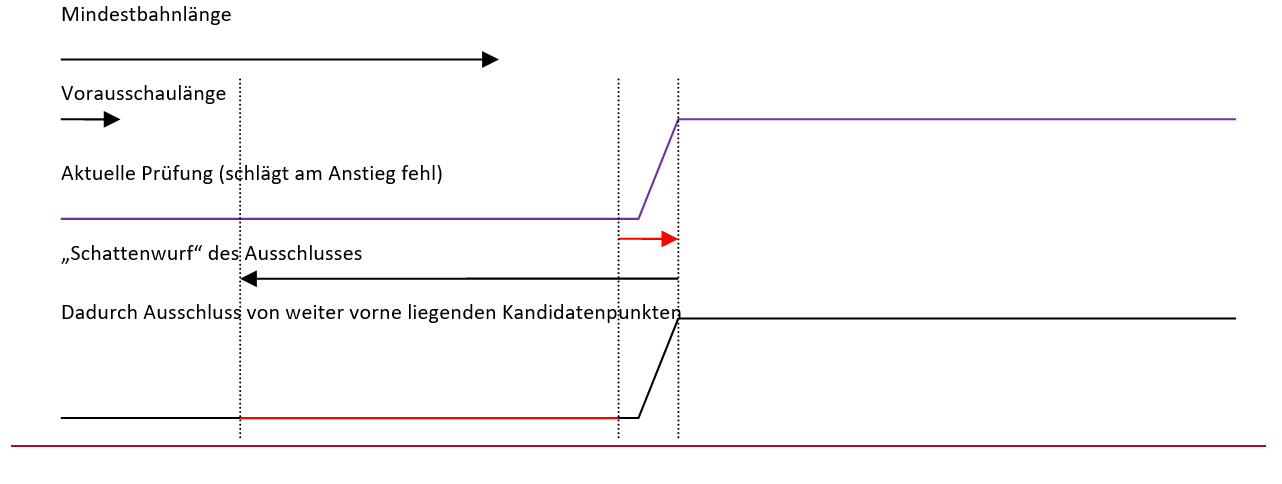
\includegraphics[width=\textwidth]{./drawings/Schattenwurf_Optimierung.png}

\begin{itemize}
\item Wenn ein Punkt aufgrund eines Kriteriums herausfällt, dann kann die direkt vor ihm liegende Strecke auf keinen Fall Teil einer geeigneten Landebahn sein. 
Es können also alle Punkte vom Ende der zugehörigen Vorausschaulänge bis zur minimalen Bahnlänge vor diesem Ende der Vorausschaulänge für weitere Berechnungen ausgeschlossen werden. Die Strecke zwischen Punkt und Vorausschauende darf dabei \emph{nicht} ausgeschlossen werden. Dort könnte ja gerade eine neue Ebene beginnen!
\item Wenn also ein ungeeigneter Punkt gefunden wird, dann brauchen die Punkte, die innerhalb der Strecke vom aktuellen Punkt bis zur Mindestbahnlänge vor dem Vorausschauende liegen nicht mehr überprüft werden.
\item Bei einer kurzen Vorausschau können also besonders viele Punkte aufgrund einer einzelnen Steigungsverletzung ausgeschlossen werden. (Fange mit den kurzen Vorausschaulängen an zu durchmustern)
\item Die Schrittweite bei jedem Durchlauf sollte also der Mindestbahnlänge entsprechen. Wenn ein Punkt herausfällt, dann werden die davor liegenden Punkte aus der weiteren Durchmusterung ausgeschlossen.
\item In einem nächsten Durchlauf wird der nächste noch zu besuchende Punkt gewählt, aber die Schrittweite bleibt bei der minimalen Bahnlänge. Wenn auf einen Punkt getroffen wird, der in einem vorherigen Durchlauf ausgeschlossen wurde, fahre mit dem Punkt fort, der eine minimale Bahnlänge Abstand vom auszulassenden Bereich hat.
\item Wiederhole so lange, bis alle Punkte entlang einer Richtung entweder ausgeschlossen wurden, oder für das überprüfte Steigungskriterium als geeignet erscheinen.

\end{itemize}
Diese Optimierung bringt nur etwas, wenn die Vorausschaulänge kleiner als die minimale Landebahnlänge ist. Bei einem wirklich „globalen“ Kriterium (Maximalanstieg auf der gesamten Bahnlänge) muss also trotzdem jeder Punkt durchmustert werden.


\subsection{Kachelränder}
Es wird der Zeitpunkt kommen, dass die betrachtete Karte nicht mehr komplett in den Speicher passt. Sei es durch Ausdehnung des Gebiets oder durch Steigerung der Auflösung. Dann muss die Karte gekachelt werden. Es ist zu klären, wie mit den Randbereichen zwischen zwei Kacheln umgegangen wird und wie es möglich wird an den Rändern zweier Kacheln zwei zu kurze Bahnen zu einer ausreichend langen zusammenzufügen. Es muss ein "`Randprotokoll"' entwickelt werden. Ein solches könnte auch zum Übergang von shared memory Systemen auf lose gekoppelte Parallelrechner (MPI) benutzt werden.

Im ersten Ansatz ist es allerdings ausreichend, wenn die auf einmal durchsuchten Kacheln ausreichend große Überlappungen aufweisen.

Bei der Durchmusterung einer Kachel müssen sowohl Anfang, als auch Ende der betrachteten Kandidatenbahn vollständig innerhalb der Kachel liegen. Daher müssen die Kacheln an den Rändern überlappen. Eine Überlappung in Größe der minimalen Bahnlänge in X- und in Y-Richtung ist ausreichend. Bei "`schräger"' Durchmusterung würde ein etwas kleinerer Überlappungsbereich ausreichen. Da aber letztendlich alle Richtungen berücksichtig werden müssen muss eine Überlappung in Größe der minimalen Bahnlänge sowohl in X- als auch in Y-Richtung hergestellt werden.

In der folgenden Grafik ist das Prinzip dargestellt: Die Länge der gezeigten Pfeile entspricht der minimalen Bahnlänge. Diese ist klein gegenüber der Gesamtausdehnung der Kacheln. Dargestellt ist die Durchmusterung der Kachel 1. Die Durchmusterung kann mit dem Fußpunkt immer auf dem Rand der aktuellen Kachel beginnen. Es muss nur so lange durchmustert werden, solange der Fußpunkt nicht im Überlappungsbereich der nächsten Kachel in Pfeilrichtung zu liegen kommt. Die rot dargestellten Pfeile sind potentielle Bahnen, die nicht bei der Durchmusterung der Kachel 1 gefunden werden können, sondern bei der Durchmusterung einer Nachbarkachel.

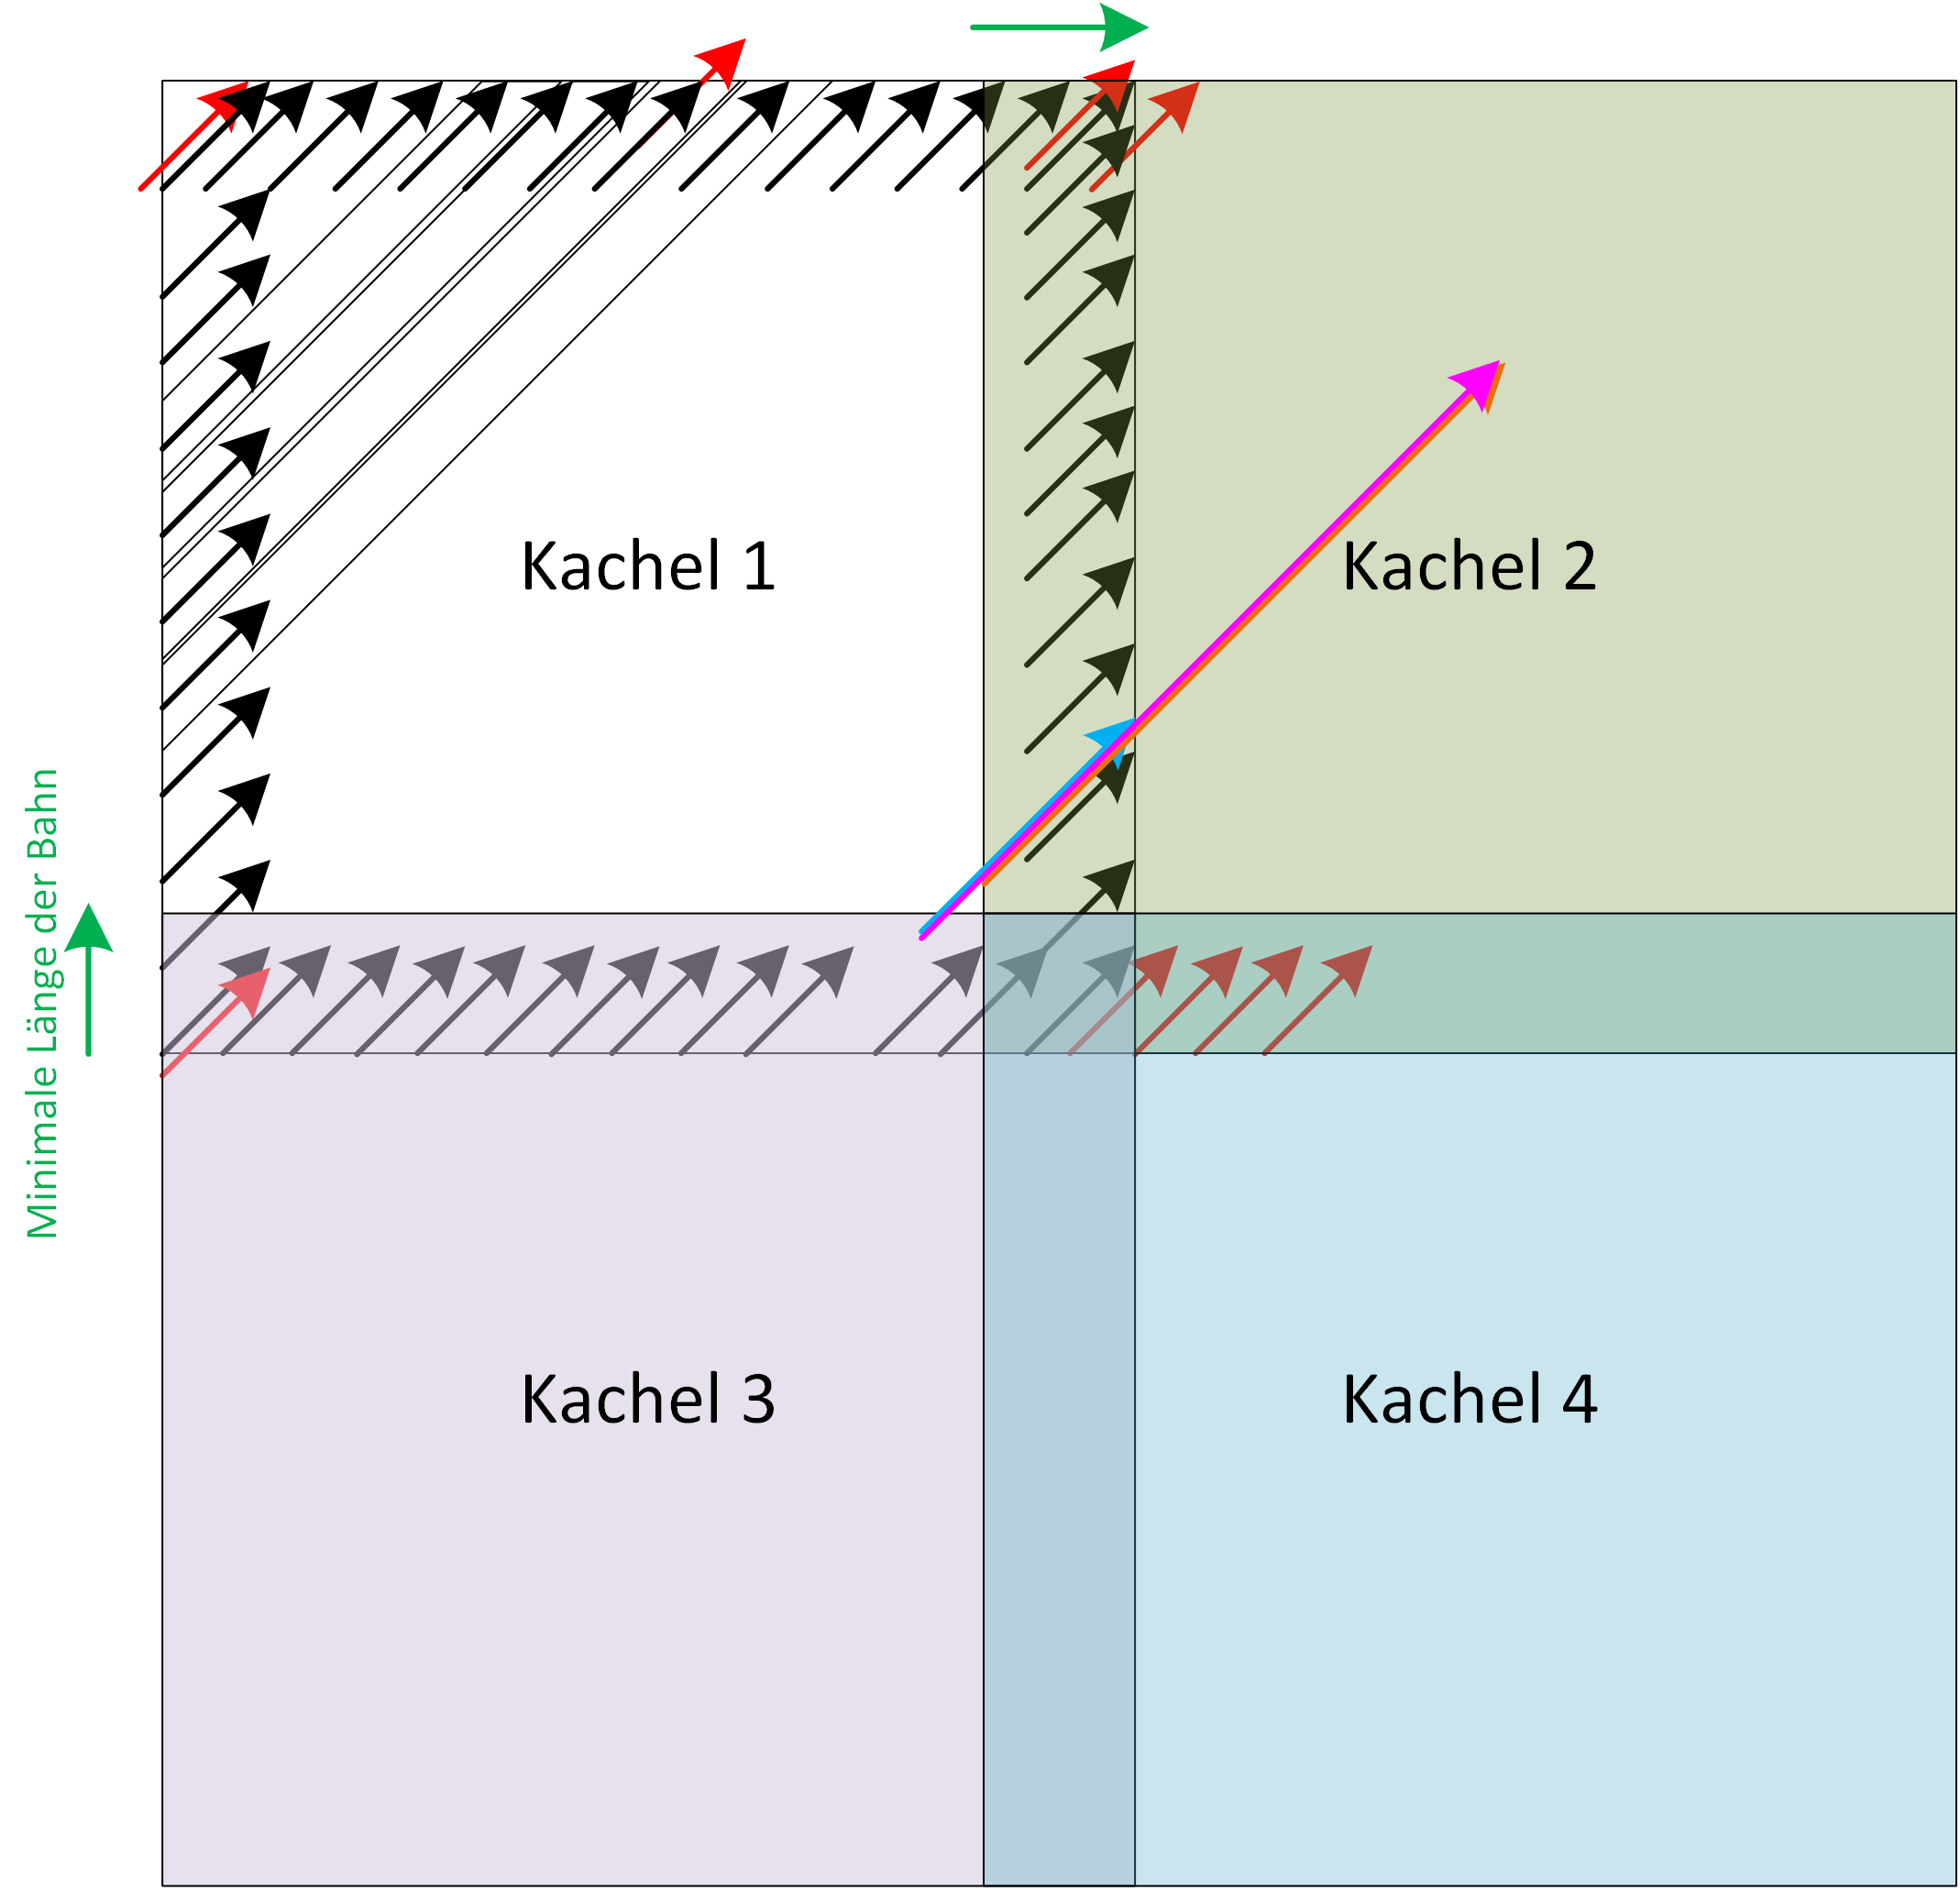
\includegraphics[width=\textwidth]{./drawings/UeberlappungKacheln.png}

Der große Vorteil eines solchen Verfahrens ist die sehr einfache Implementierung. Dem stehen zwei Nachteile entgegen:
\begin{itemize}
	\item Die Übberlappungsbereiche müssen zweimal in den Speicher geladen werden. Einige Tests werden im Überlappungsbereich doppelt ausgeführt. Das ist nicht schlimm, solange die Kacheln groß gegenüber dem Überlappungsbereich sind. Davon kann in der Praxis ausgegangen werden.
	\item Eine lange Bahn (in der Grafik pink) wird nicht als eine einzelne lange Bahn, sondern als zwei einzelne (in der Grafik hellblau und ocker) überlappende Bahnen erkannt. Auch das ist nicht schlimm, da jede einzeln für sich genommen noch lang genug ist und daher als Notlandebahn in Frage kommt.
\end{itemize}


\subsection{Datenstrukturen während der Durchmusterung}

Wie bereits im Abschnitt \ref{Einfache_Durchmusterung} erwähnt, kann aus dem Ausschluss eines Punktes auf Grund der Verletzung eines Kriteriums beim Durchmustern in einer beliebigen Richtung $a$ nicht unmittelbar geschlossen werden, dass dieser Punkt nicht Teil einer Landbahn in einer weiteren Richtung $b$ sein. Das kann man sich gut an dem Extremfall einer steilen Geländekante verdeutlichen: Orthogonal zur Geländekante reißen zwei benachbarte Punkte das Holprigskeitskriterium, doch können beide Punkte jeweils Teil einer Landebahn parallel zu dieser Geländekante sein.
Aus diesen Überlegungen resultiert, dass auch, wenn mehrere Threads ein und dieselbe Geländekachel bearbeiten, sie relativ wenige nützliche Befunde sinnvoll teilen / verwenden können. Da die Implementation auch das Vorgegeben beliebiger Durchmusterungswinkel zulässt, sollte jeder Thread ein separates Objekt pflegen, in dem er lokale Informationen ablegen und Geländepunktinformationen speichern kann. 
Einen Sonderfall stellen sicher die Kartengeopunkte selbst dar. Diese werden von allen Threads lediglich lesend benötigt. Da diese zudem die sicherlich größte persistente Datenmenge darstellen, ist darauf zu achten, diese nur möglichst kurz und nicht mehrfach im Speicher zu halten sind. Deswegen ist die Idee, eine Klasse zu implementieren, die sich ausschließlich mit der Verwaltung der Daten im Speicher (also einlesen und freigeben, Darstellung von NICHT-Kartenpunkten / NULL - Werte an Kartenrändern ) beschäftigt, während die Threads einen Zeiger/Referenz auf dieses Datenobjekt besitzen. Es muss sichergestellt werden, dass so lange ein Thread noch Zugriff auf eine Kachel benötigt, diese auch noch verfügbar sein muss. Zum jetzigen Zeitpunkt ist noch nicht völlig überschaubar, welche zusätzlichen Daten bei der Durchmusterung vorgehalten werden müssen. Dieses wird aber sicherlich in das Datenobjekt der Klasse einfließen.

\section{Datenhaltung gefundener Notlandeflächen}

Gefundene Landebahnen sind Rechtecke. Entlang eines Durchmusterungsstrahls werden maximal lange Rechtecke mit der gewünschten Landebahnbreite gefunden. Die Wahrscheinlichkeit ist sehr hoch, dass auf nebeneinander laufenden parallelen Durchmusterungen auch nebeneinanderliegende parallele Landebahnen gefunden werden. Diese überlappen sich in der Regel. 

Der einfachste und in ersten Prototypen zu beschreitende Weg wäre es, jede dieser überlappenden Bahnen einzeln in die Datenbank einzutragen und einzeln zu behandeln. Dazu reicht der Start- und der Endpunkt der Bahn aus. Die Bahn liegt dann um diese Mittellinie herum mit der geforderten Breite.

Dies führt aber zu sehr vielen Einträgen und macht die Ergebnisse unübersichtlich.

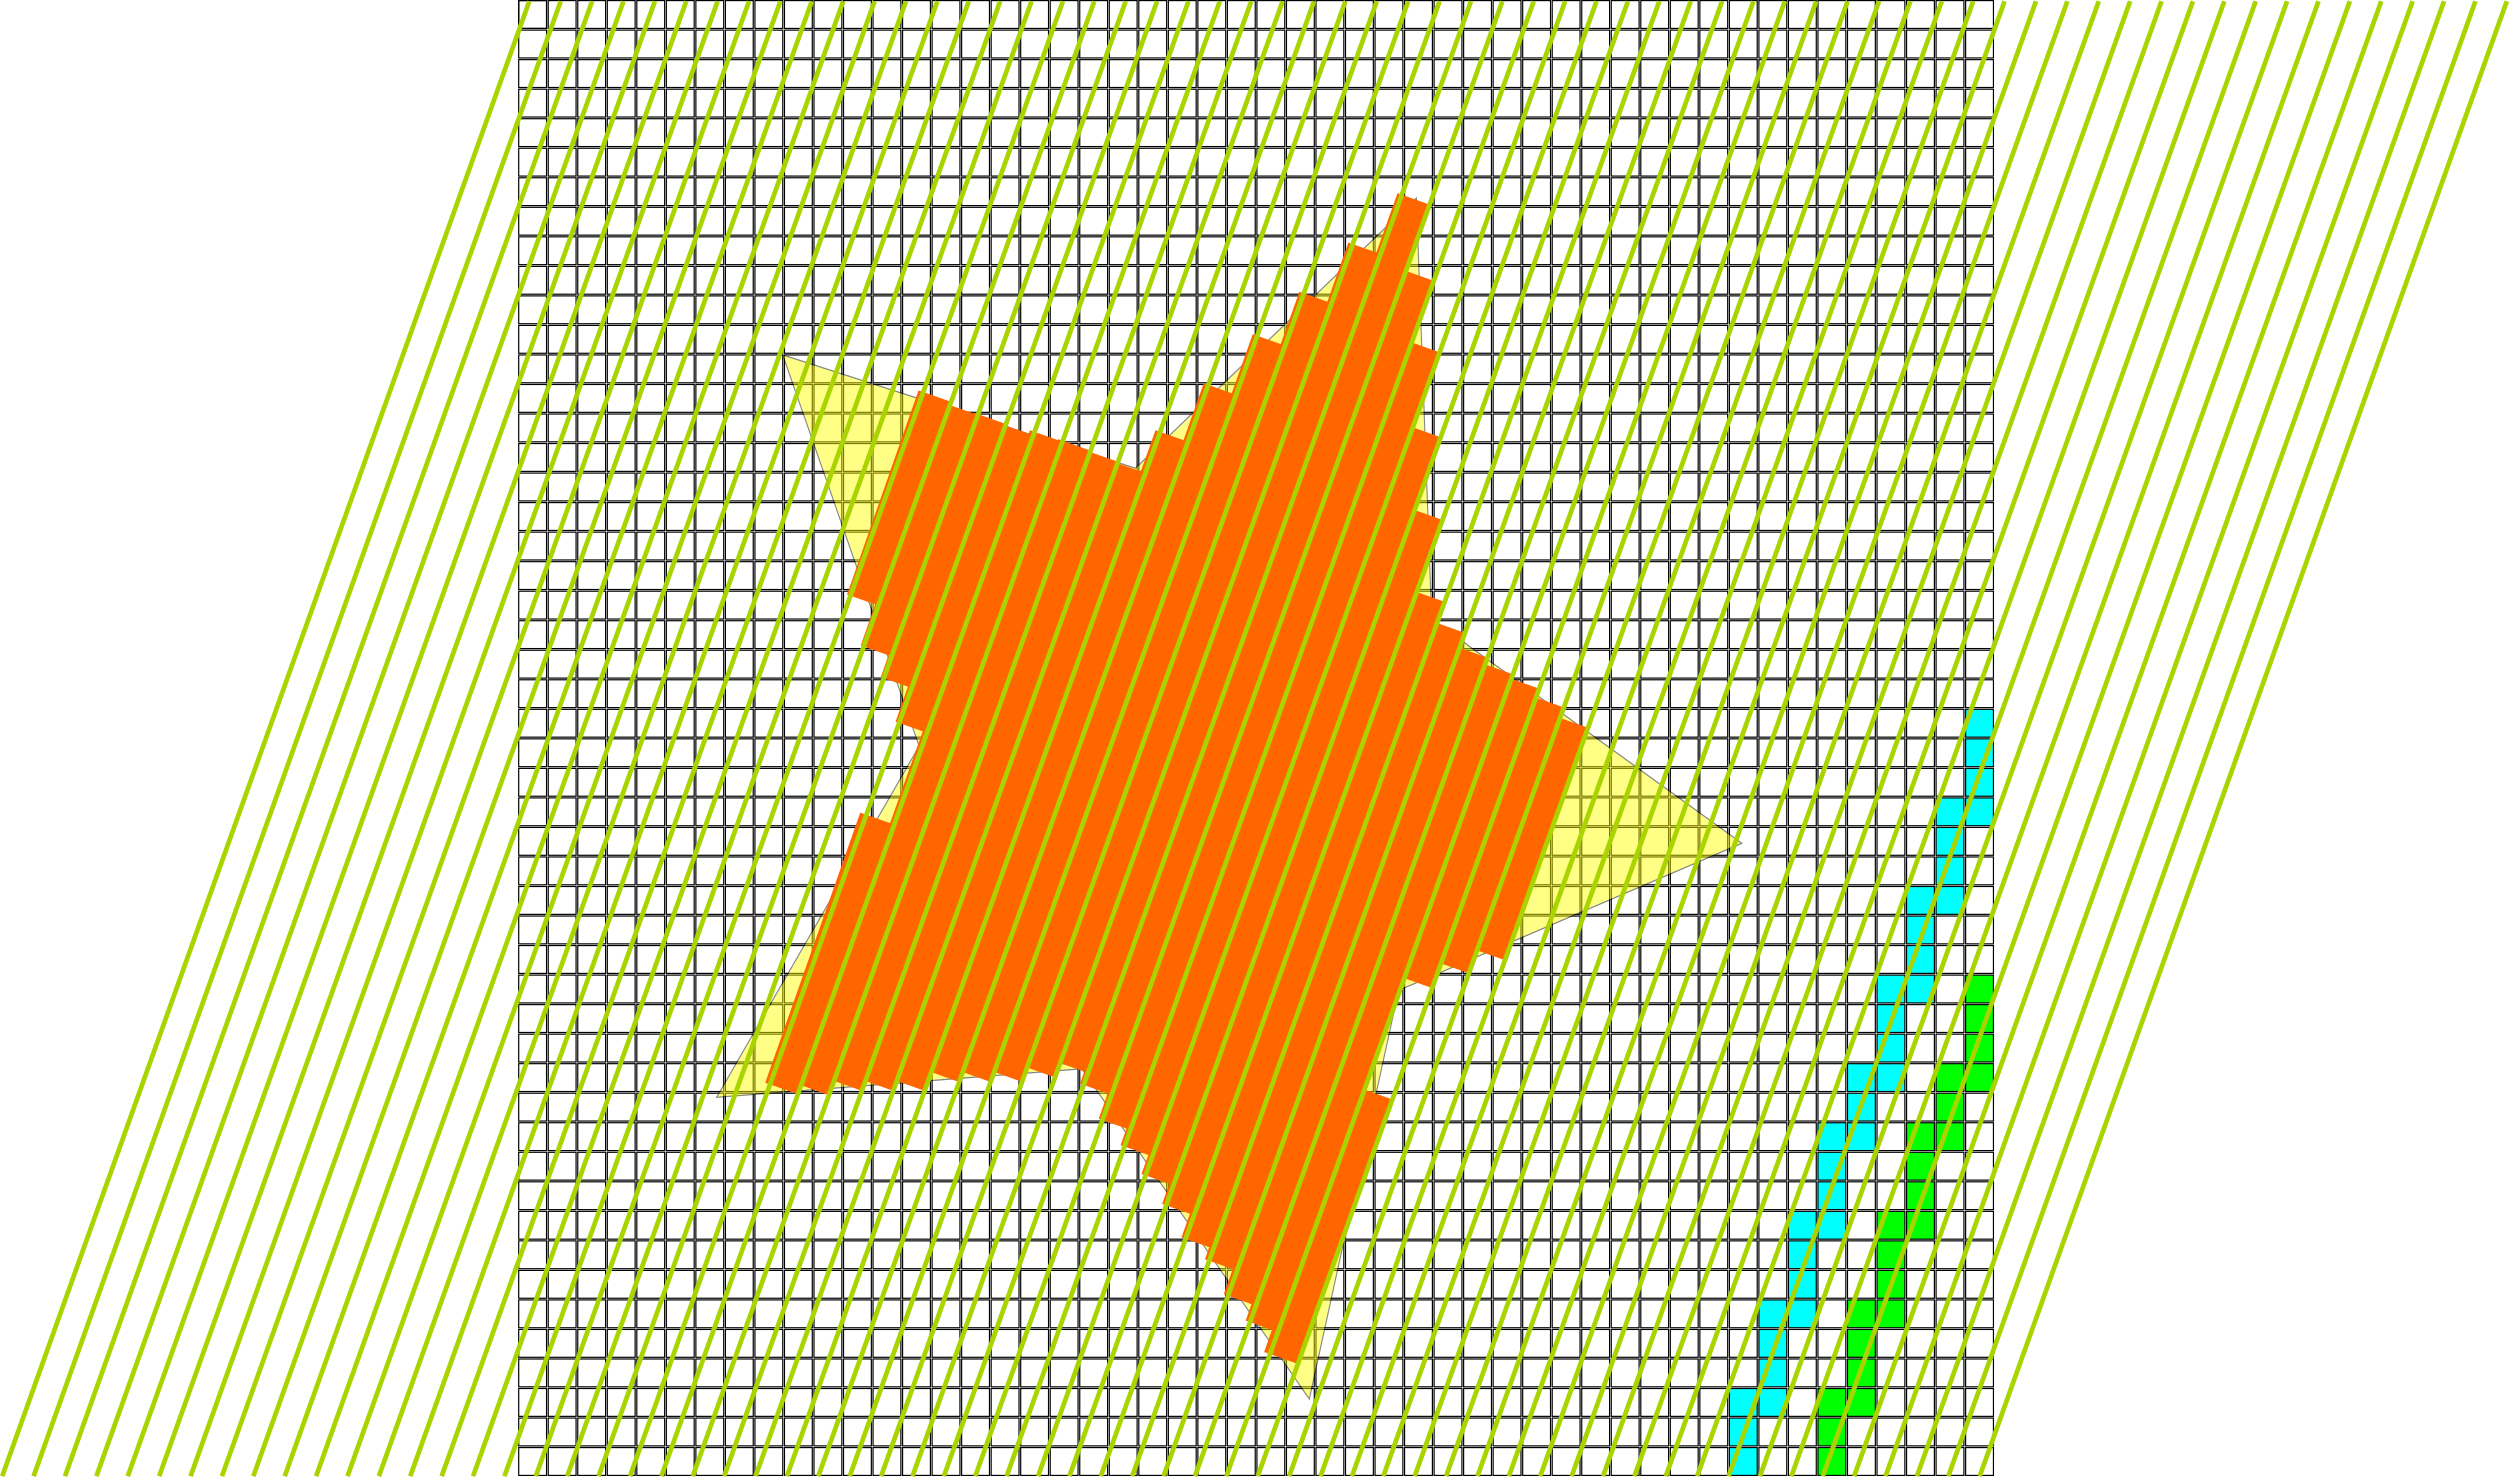
\includegraphics[width=\textwidth]{./drawings/ueberlappendeBahnen.png}

Besser wäre es, wenn sich überlappende Bahnen zu einer einzigen Landefläche mit einem Polygonumriss zusammengefasst werden. 

\subsection{Auswahl der Datenbank}

Es soll eine Datenbank ausgewählt werden, die Geodaten unterstützt. Offenbar hat sich als Format für Geo-Daten das Format \href{http://geojson.org/}{GeoJSON} etabliert. Eine Datenbank, die dieses Format und spezielle Abfragen darauf unterstützt ist z. B. \href{https://docs.mongodb.com/}{MongoDB}.

In diese Datenbank sollen gefundene Landeflächen als Polygonumriss mit ihrer Richtung eingetragen werden.

MongoDB unterstützt unter anderem auch direkte geographische Abfragen, so dass auch eine Abfrage nach allen Notlandeflächen in maximal 20km Entfernung recht leicht möglich sind. Siehe dazu \href{https://docs.mongodb.com/manual/reference/operator/query-geospatial/}{Geospatial Query Operators}.

\subsection{Merge von überlappenden Notlandebahnen}

MongoDB unterstützt auch eine Abfrage \href{https://docs.mongodb.com/manual/reference/operator/query/geoIntersects/#op._S_geoIntersects}{\texttt{\$geoIntersects}}. Damit ist es möglich, beim Eintrag einer neuen Landefläche direkt abzufragen, ob diese neue Fläche mit bereits vorhandenen Objekten in der Datenbank überlappt. 

Falls dies der Fall ist, können alle überlappenden Landeflächen einer Richtung zu einem gemeinsamen Objekt zusammengefasst werden. Diese Zusammenfassung kann in einem eigenen Prozess durchgeführt werden. 

Der genaue Algorithmus zum Merge mehrerer Polygone muss noch erarbeitet werden. Dabei kann man sich zunutze machen, dass die Rechtecke einer einzelnen Bahn immer entlang der Durchmusterungsrichtung verlaufen und nur dazu senkrechte und parallele Linien vorkommen können. 

\section{Benutzung und Visualisierung}

Da die Programmierung einer Visualisierung und einer GUI erfahrungsgemäß eine Qual ist, soll möglichst auf vorhandene Standardtechnologien zurückgegriffen werden.

Es bietet sich an, das System über einen Webbrowser zu steuern. Dazu sind im Wesentlichen zwei Funktionen notwendig:
\begin{itemize}
	\item Auswahl des zu untersuchenden Kartenausschnitts
	\item Darstellung der gefundenen Landeflächen auf einer Karte
\end{itemize}

Es bietet sich an auf die frei verfügbaren Daten und die Visualisierung von OpenStreetmap (OSM) zurückzugreifen. 

Zur Bereichsauswahl des zu durchmusternden Bereichs soll die Ausdehnung/Überdeckung eines Datensatzes als Overlay in OSM eingeblendet werden. (TODO: entscheide, ob lediglich die rechteckige Bounding Box der Koordinaten, oder aber die echte Kontur eingeblendet werden soll.)
In OSM kann mittels \href{http://wiki.openstreetmap.org/wiki/Bounding_Box}{"`boundingBox"'} eine Auswahl erfolgen. Es wird ein Rechteck in Geo-Koordinaten zurückgegeben. Wenn diese Geo-Koordinaten in Pixel umgerechnet sind, dann kann der entsprechende Bereich –entweder am Stück, oder gekachelt– eingelesen und durchmustert werden. 

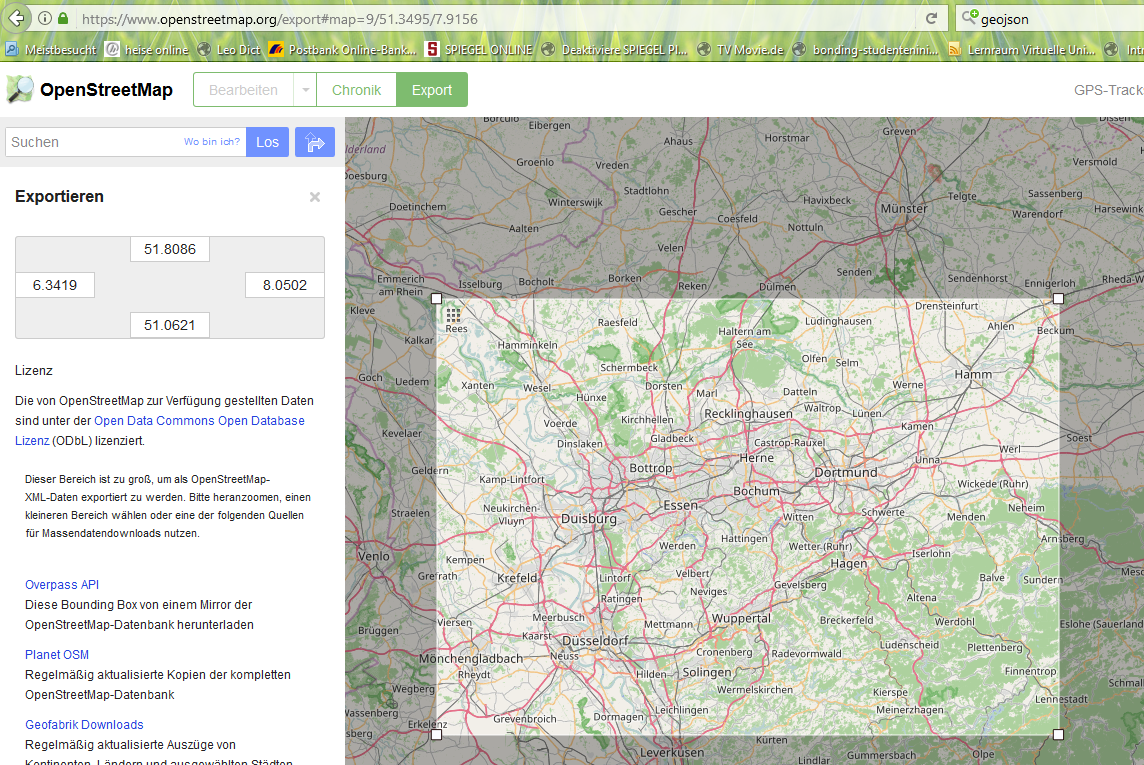
\includegraphics[width=\textwidth]{./drawings/AuswahlKartenausschnitt.png}

Für die Visualisierung bietet sich eine kleine JavaScript-Anwendung an, die die Darstellung im Browser übernimmt. Damit kann auf Standardtechnologien zurückgegriffen werden und es muss nicht zu viel Hirnschmalz in die Visualisierung und eine Benutzeroberfläche gesteckt werden. 
Eine JavaScript-Webseite kann selbständig auf die Datenbank zugreifen und so die gefundenen Landeflächen in OSM als Polygone in die Karte einblenden. 

Als Bibliothek zur Realisierung einer solchen Funktionalität scheint \href{http://leafletjs.com/examples.html }{Leaflet} geignet und ausreichend leicht in der Benutzung.





\section{Parallelisierung}

\subsection{Feinkörnige Parallelisierung der Durchmusterung mit pthreads}

Bei relativ wenigen Threads und relativ viel Speicher kann jeder Thread eine Kachel in einer Richtung komplett durchmustern. Da auf die Eingabedaten nur lesend zugegriffen wird und die Durchmusterungen in unterschiedlichen Richtungen unabhängig sind, braucht man sich keinerlei Gedanken über die Synchronisierung des Speicherzugriffs machen. Es muss lediglich eine Barrier eingerichtet werden, bevor die nächste Kachel in den Speicher geladen wird.

Nachteilig bei diesem Verfahren ist leider der recht hohe Speicherbedarf, da bei x Threads auch x mal Speicher für die Zwischendaten reserviert werden muss.

\skippingparagraph

Bei genauerer Betrachtung fällt auf, dass nicht nur die einzelnen Richtungen bei der Durchmusterung vollständig unabhängig voneinander sind, sondern auch die Durchmusterung entlang jedes einzelnen Durchmusterungsstrahls. Das heißt, dass es leicht möglich ist, jedem Thread die Durchmusterung entlang eines einzelnen Durchmusterungsstrahls aufzugeben. Bei bekannter Anzahl der Threads kann im voraus statisch festgelegt werden, welcher Thread sich entlang welchen Strahls bewegen soll. Laufzeitmessungen in der Praxis können zeigen, ob ein dynamischer Workpoolansatz notwendig ist um die Last besser aufzuteilen. Intuitiv scheint das nicht notwendig, da nicht zu erwarten ist, dass die einzelnen Durchmusterungen sehr große Schwankungen bezüglich der Rechenzeiten aufweisen. Die Praxis wird zeigen, ob diese Annahme korrekt ist.
Zur Verbesserung des Speed-Ups ist angedacht, die Parallelisierung dahingehend zu verbessern, dass Threads, die in der aktuellen Kachel nichts mehr zu erledigen haben bereits mit dem Durchmustern der nächsten Kachel beginnen können. Dies könnte man leicht unter Zuhilfenahme eines Semaphores erreichen (entfernen der vorhin angedeuten Barrier). Hier ist allerdings zu evaluieren, wie sich die Hinzunahme weiterer Kacheln in den Speicher auf dessen Verbrauch auswirkt. Im Worst-Case könnten bei $n$-Threads $n$-Kacheln im Speicher gehalten werden müssen.


	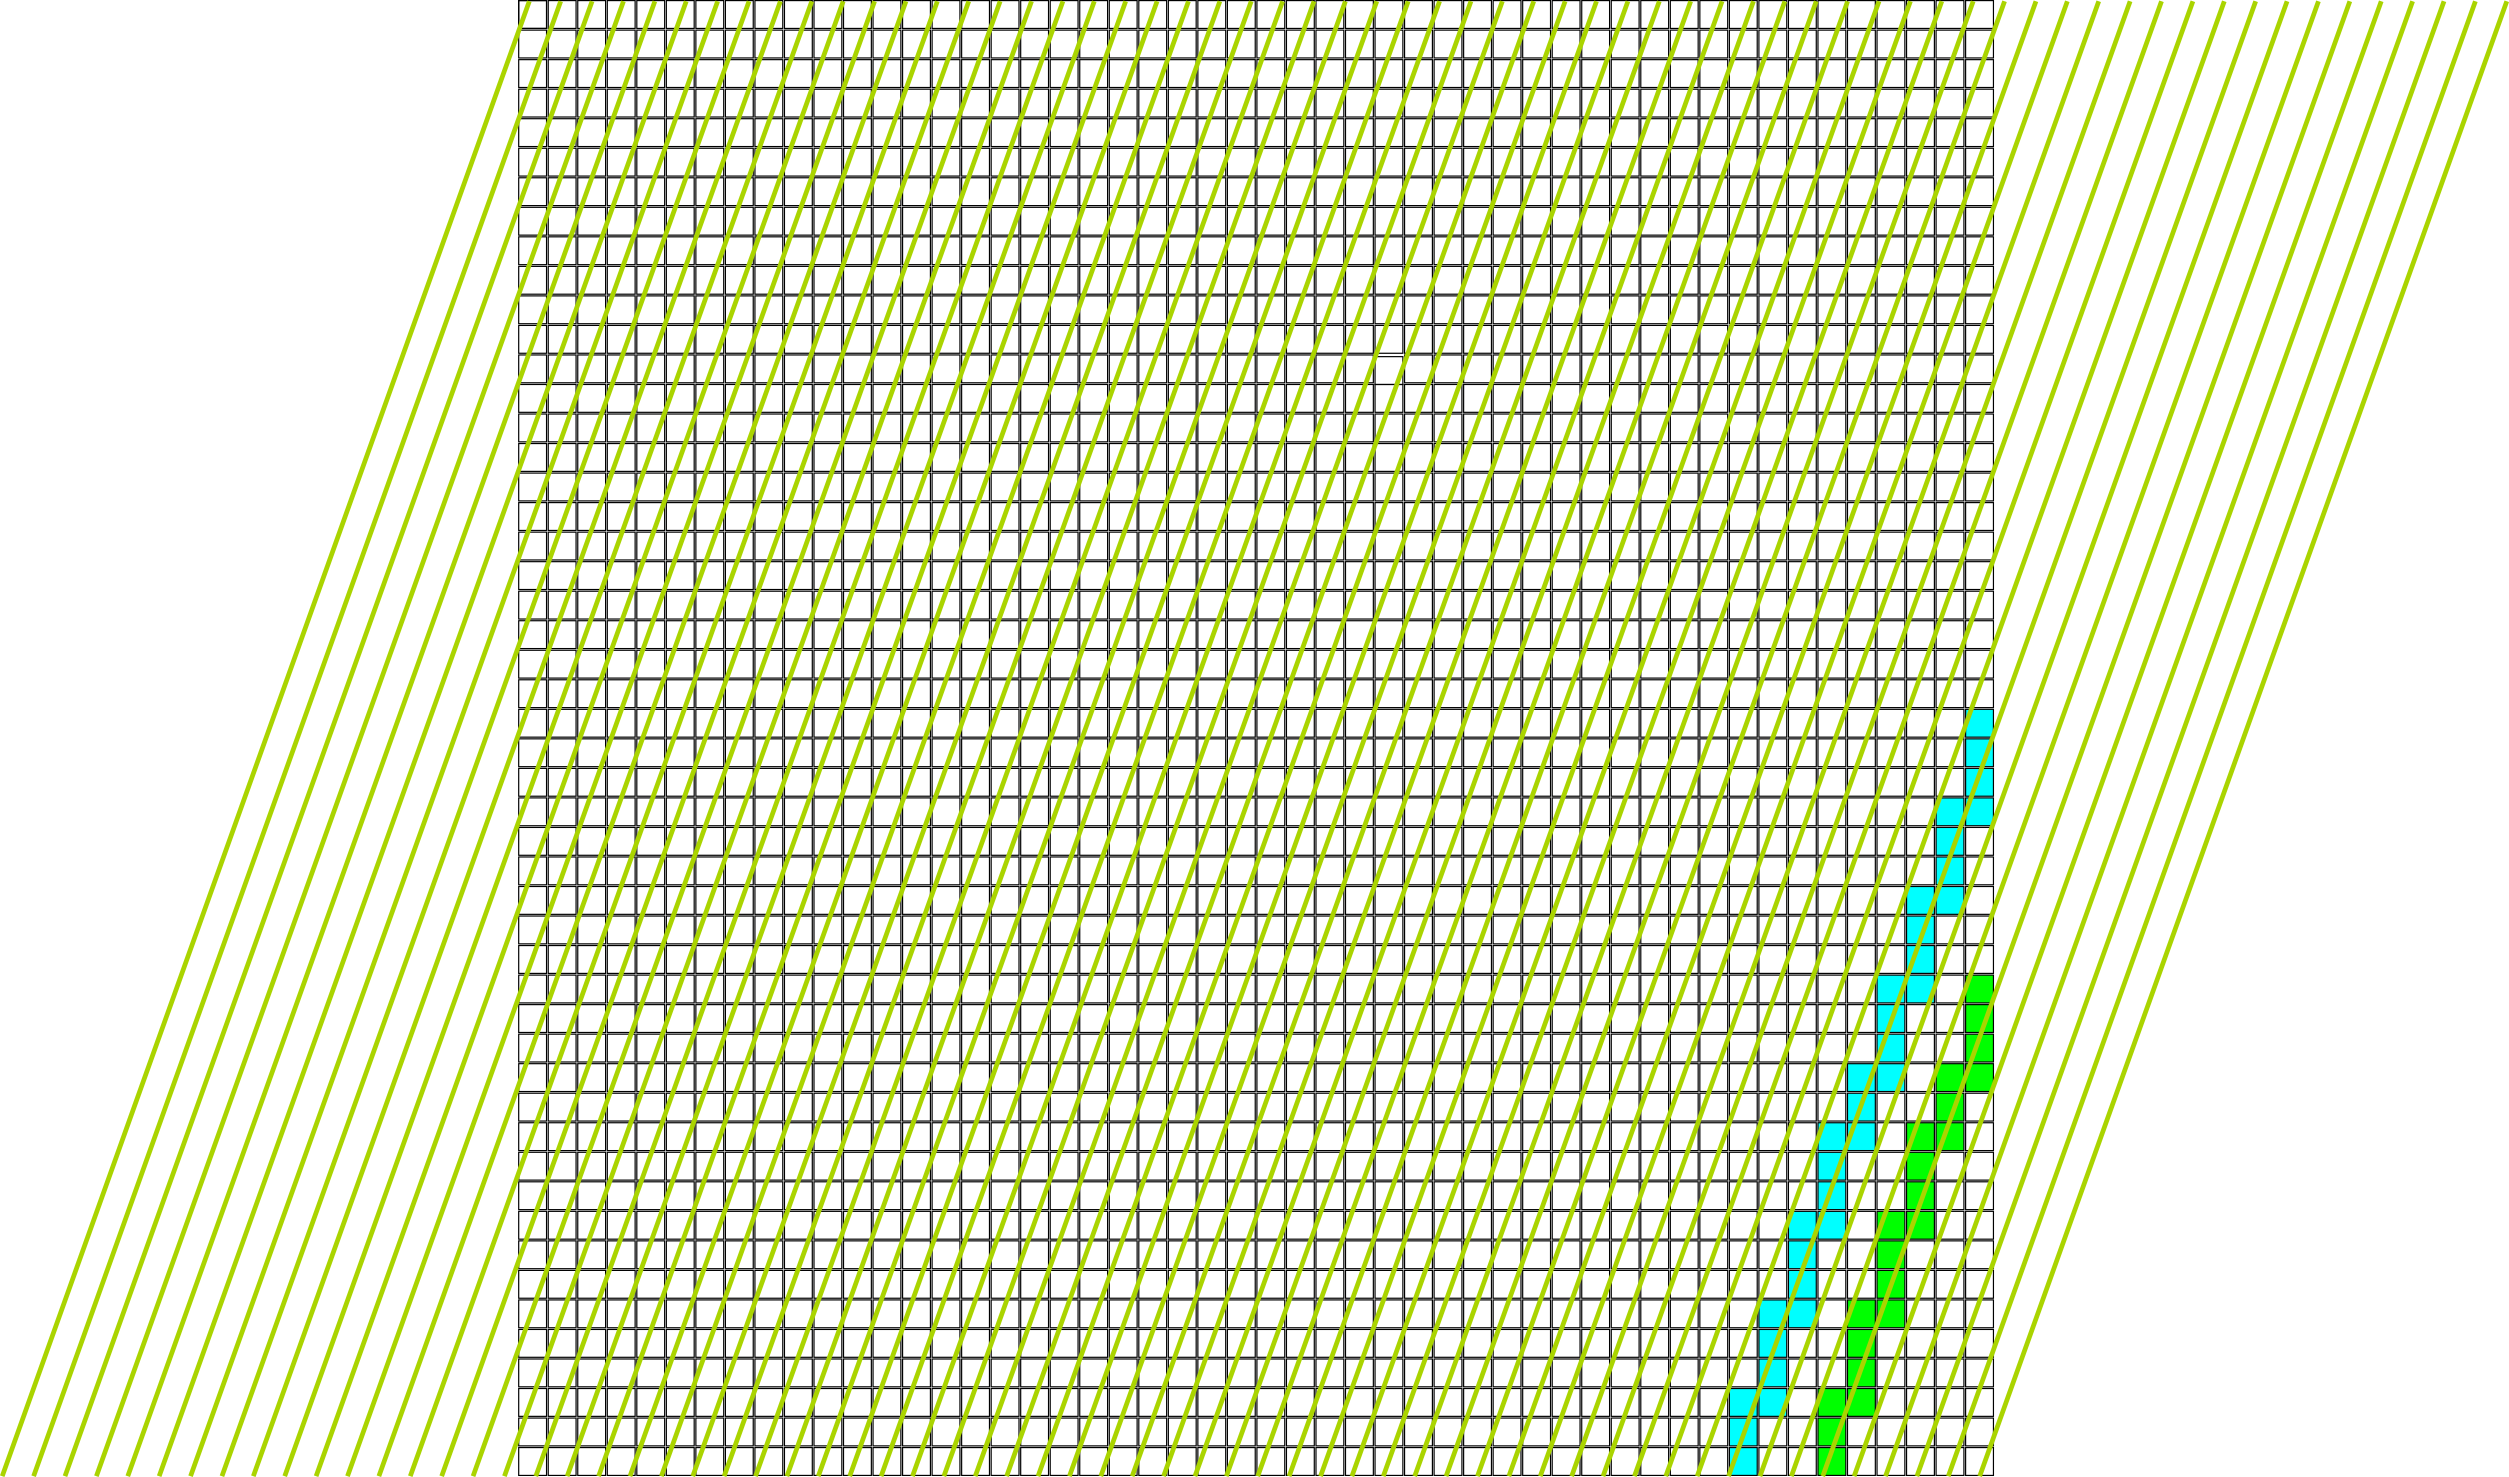
\includegraphics[width=0.5\textwidth]{./drawings/Durchmusterungspfade_schraeg.png}

\subsection{Grobkörnige Parallelisierung verschiedener Programmteile mit mehreren Prozessen}
Neben der angesprochenen feinkörnigen Paralleliserung sind noch weitere grobkörnigere Paralleisierungen im geplanten System implementiert:
\begin{itemize}
	\item Auswahl des zu durchmusternden Bereichs per Webinterface
	\item Eintrag der gefundenen Landeflächen in die Datenbank 
	\item Merge überlappender Notlandebahnen zu einer Polygonfläche
	\item Visualisierung der gefundenen Ergebnisse per Webinterface
	\item (Wenn noch Zeit zur Implementierung: Abgleich der gefundenen Landeflächen mit OpenStreetmap Daten zum weiteren Filtern von Verbostzonen wie z. B. Seen oder Autobahnen)
\end{itemize}

\end{document}